% Editorially assembled from the preserved September 17 report.
\section{Preliminaries and the estimator}\label{sec:preliminaries}
Let $A\in\mathbb R^{d\times d}$ be fixed and real symmetric. Positive semidefiniteness is needed for the ordered positive-eigenvalue models, but not for the trace and variance identities. Let $Q\in\mathbb R^{d\times r}$ have orthonormal columns. Empty $Q$ is permitted. Define


\begin{equation}
R_Q=I-QQ^\top,\qquad H_Q=R_QAR_Q.
\end{equation}


These matrices are mathematical objects; production implementations apply the projectors implicitly rather than materializing dense residual matrices.


{\small
\begin{longtable}{@{}>{\raggedright\arraybackslash}p{0.1848\linewidth}>{\raggedright\arraybackslash}p{0.6952\linewidth}@{}}
\caption{Notation and conditioning}\label{tab:auto1}\\
\toprule
Symbol & Meaning and distinction \\
\midrule
\endfirsthead
\toprule
Symbol & Meaning and distinction \\
\midrule
\endhead
$m$ & Total estimator query budget \\
$S$ & Range-sketch matrix; uppercase $S$ is reserved for this object \\
$q$ & Attempted sketch columns / products forming $AS$ \\
$r=r_q$ & Accepted basis rank; $r\le q$, not automatically $q$ \\
$k=r_\star$ & Dominant rank in a synthetic step model, not accepted rank \\
$B$ & Stopped reusable pilot width; $B\le q$ \\
$\ell$ & Fresh final residual-probe count \\
$s$ & Fresh certification-probe count, separate from $\ell$ \\
$c_{\rm pre}$ & Actual committed candidate-construction cost \\
$\mathcal F$ & Information fixing candidate actions before certification \\
$\mathcal G$ & Information fixing the selected action before final estimation, including certification if used \\
$\widehat\sigma_{x,s}^{\,2}$ & Unbiased sample variance for action $x$ from $s$ certification probes \\
\bottomrule
\end{longtable}
}
Conditioning on $\mathcal F$ or $\mathcal G$ freezes the corresponding actions and their residual denominators. Fresh probes are independent of that information and conditionally iid. A random pilot stage or allocation is allowed; freshness, rather than a deterministic stopping time, is the essential condition.

\begin{proposition}[Exact construction accounting]\label{thm:T1}
Pilot products are retained inside the final $q$-column range sketch. An accepted $r$-column basis is used, and $AQ$ is queried once and cached. No additional oracle calls are omitted from the ledger.


The basic architecture has


\begin{equation}
\boxed{q+r+\ell=m,\qquad \ell=m-q-r>0.}
\end{equation}


The special case $\ell=m-2q$ holds only when $r=q$. A rejected sketch direction costs one query even when it gains no rank.


\end{proposition}
\begin{proof}
A reusable pilot of width $B$ followed by $q-B$ new columns costs $B+(q-B)=q$, not $B+q$. Computing $AQ$ costs $r$ additional products, and final residual estimation costs $\ell$. Adding these disjoint costs gives the identity. There is no cancellation of an attempted query merely because QR rejects its direction.

\end{proof}


Retaining a pilot of width $B$ restricts the final sketch to $q\ge B$. For nested candidates sharing all required products, $c_{\rm pre}=\max_x(q_x+r_x)$; otherwise, $c_{\rm pre}$ is the actual committed query count.


\begin{figure}[tbp]
\centering
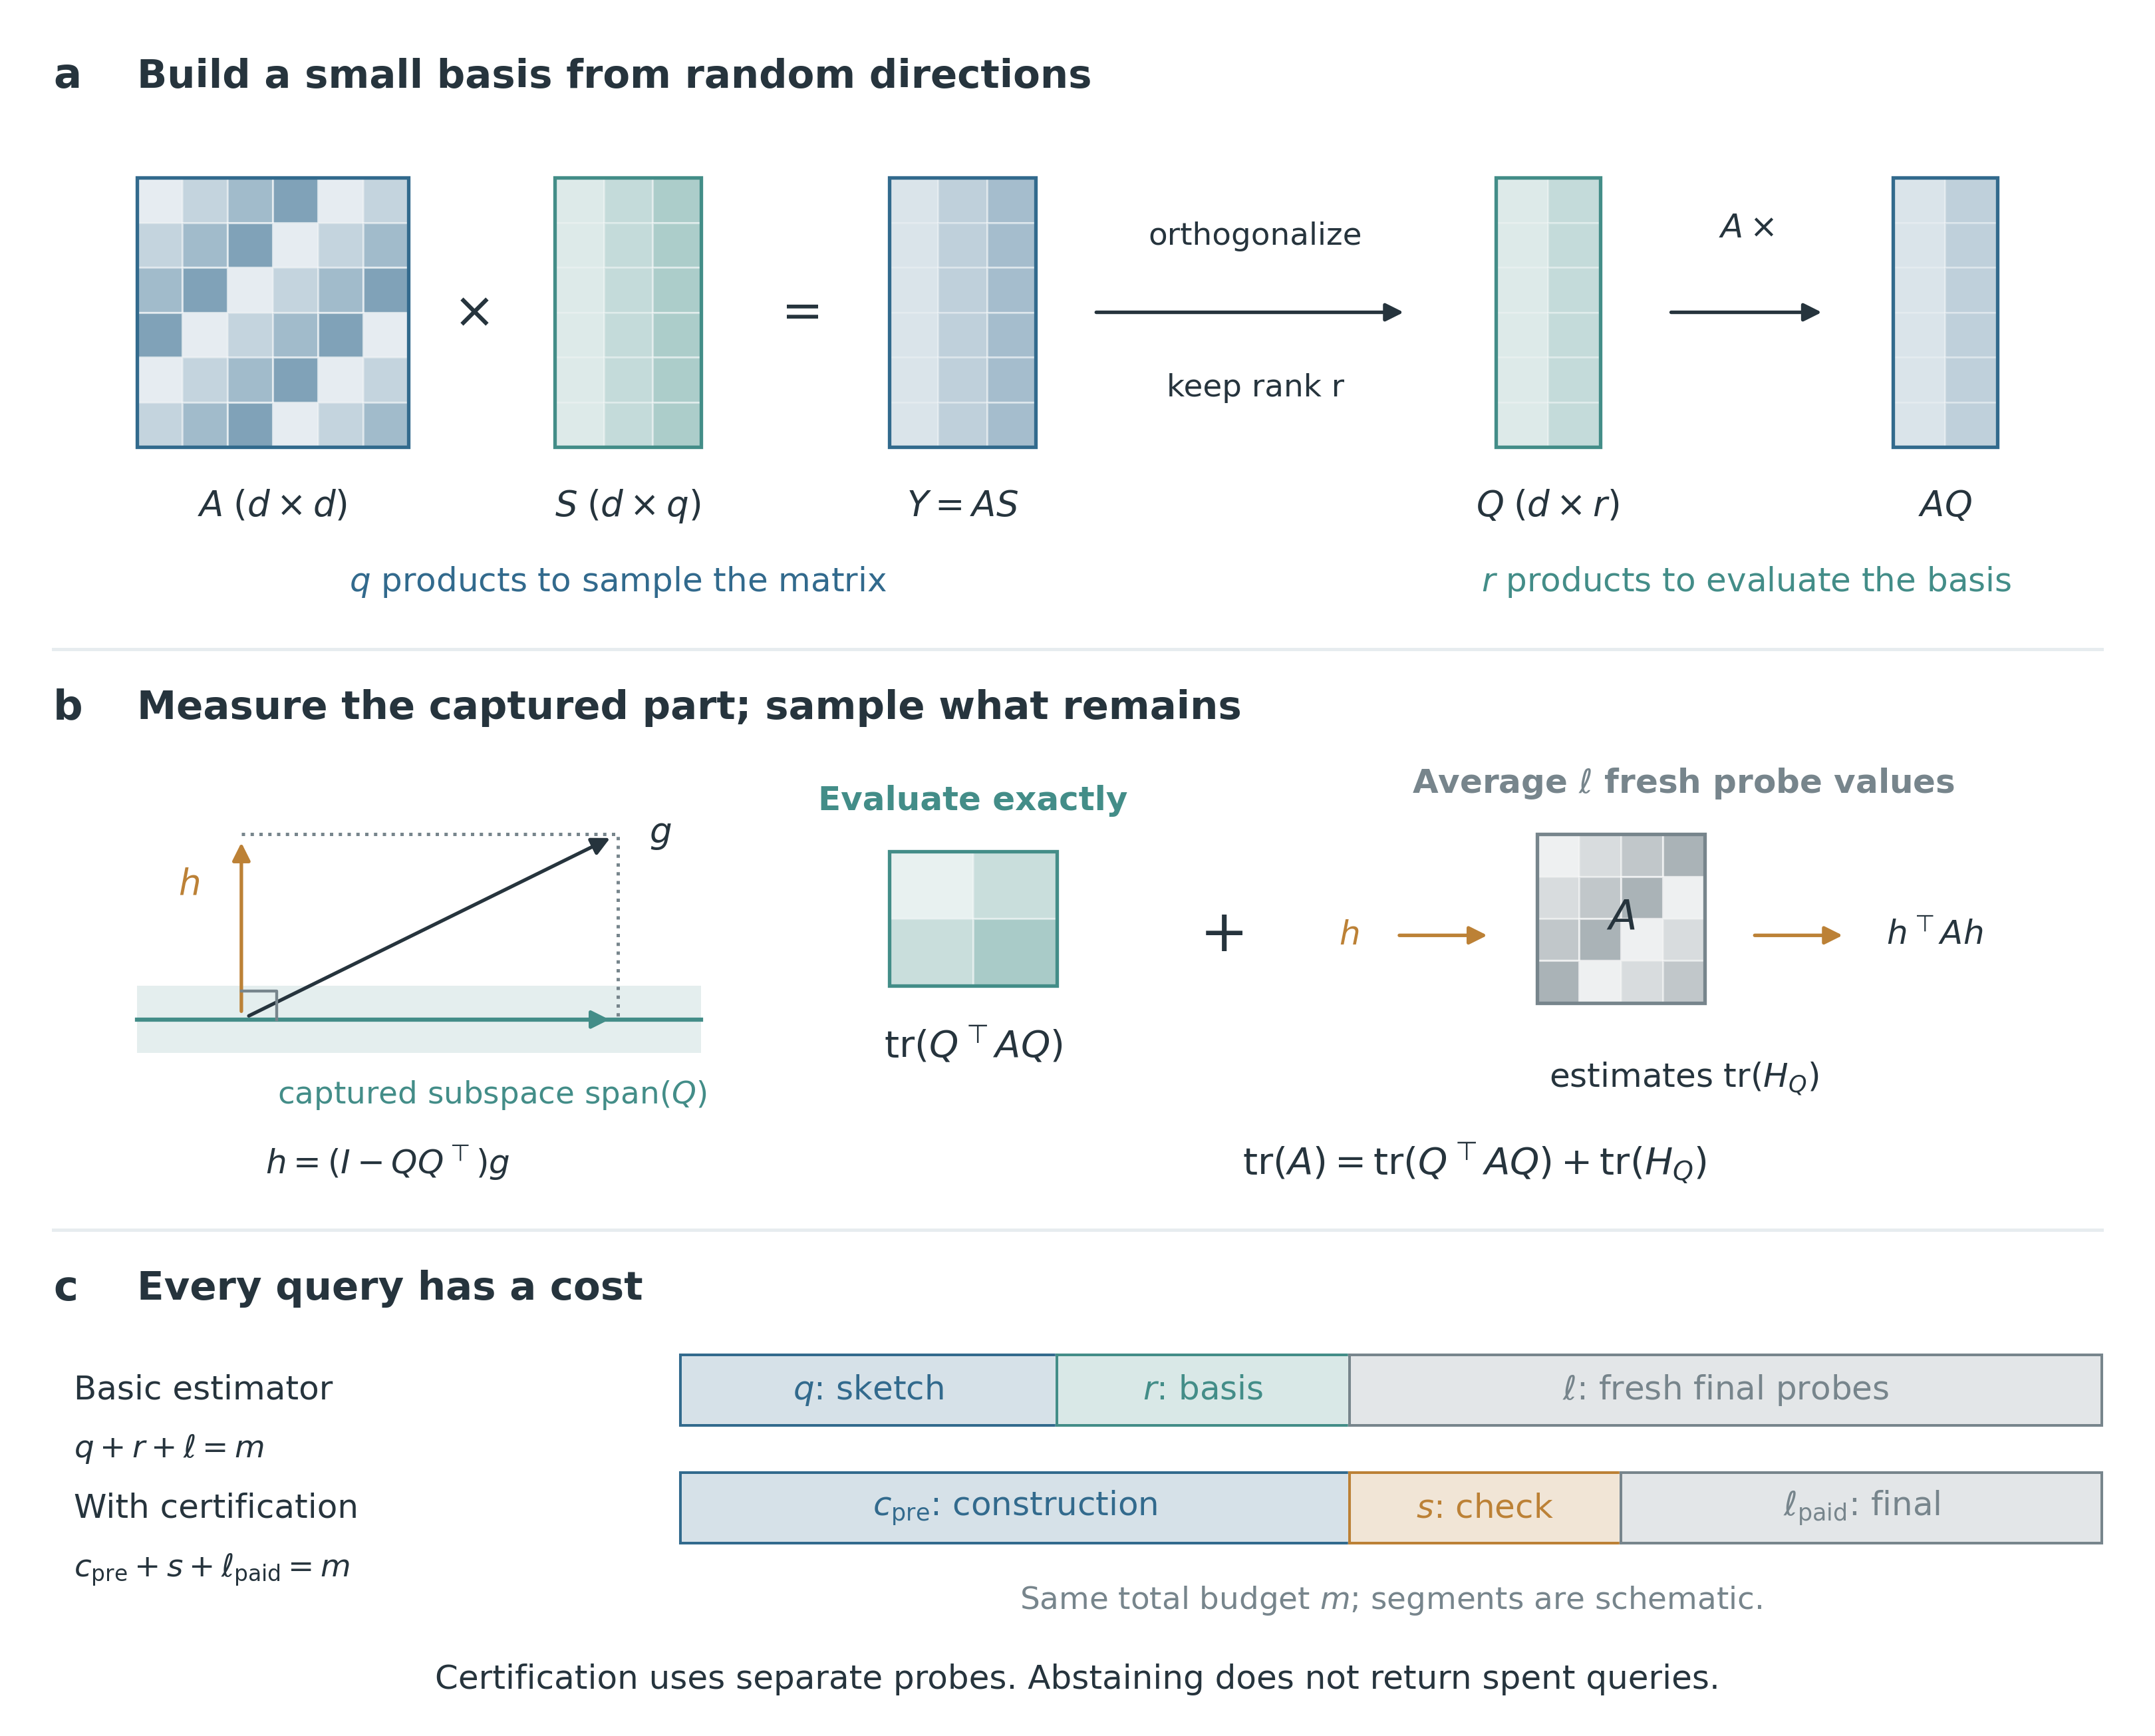
\includegraphics[width=\linewidth]{figures/workflow.png}
\caption[What each query buys]{\textbf{What each query buys.} (a) A random sketch constructs a basis with accepted rank $r\le q$; evaluating $AQ$ costs another $r$ queries. (b) The captured trace contribution is evaluated exactly, while fresh projected probes estimate the complementary trace. The geometry is schematic and does not assert exact dominant-eigenspace capture. (c) Certification consumes $s$ additional queries, leaving $\ell_{\rm paid}=m-c_{\rm pre}-s$. Bar widths are schematic. Returning to a baseline basis does not refund committed queries.}
\label{fig:workflow}
\end{figure}

\begin{algorithm}
\caption{Frozen-action trace estimation: accounting template}\label{alg:frozen}
\textbf{Input:} symmetric matrix--vector oracle, budget $m$, a range policy using $q$ products.\\
\textbf{Output:} an unbiased trace estimate, provided $\ell=m-q-r>0$.
\begin{enumerate}
\item Construct $AS$ with $q$ oracle products, retaining any reusable pilot prefix.
\item Compute an orthonormal accepted basis $Q$ of rank $r$ and query/cache $AQ$ with $r$ products.
\item Freeze the action and set $\ell=m-q-r$.
\item Draw $\ell$ fresh independent isotropic probes $g_j$.
\item Form $h_j=g_j-Q(Q^\top g_j)$, query $Ah_j$, and return
$\tr(Q^\top AQ)+\ell^{-1}\sum_j h_j^\top Ah_j$.
\end{enumerate}
\end{algorithm}
\begin{theorem}[Conditional unbiasedness, including sequential decisions]\label{thm:T2}
$Q$ and the positive integer $\ell$ are $\mathcal G$-measurable. Each final probe satisfies $\mathbb E[g_jg_j^\top\mid\mathcal G]=I$. The requisite expectations exist.


For


\begin{equation}
\widehat t=\operatorname{tr}(Q^\top AQ)+\frac1\ell\sum_{j=1}^{\ell}g_j^\top H_Qg_j,
\end{equation}


we have


\begin{equation}
\mathbb E[\widehat t\mid\mathcal G]=\operatorname{tr}(A),\qquad
\mathbb E\widehat t=\operatorname{tr}(A).
\end{equation}


\end{theorem}
\begin{proof}
Conditional isotropy gives $\mathbb E[g_j^\top H_Qg_j\mid\mathcal G]=\operatorname{tr}(H_Q)$. Because $R_Q^2=R_Q$, cyclicity of trace yields


\begin{equation}
\operatorname{tr}(H_Q)=\operatorname{tr}(AR_Q)
=\operatorname{tr}(A)-\operatorname{tr}(Q^\top AQ).
\end{equation}


Thus the two pieces of the estimator add in conditional expectation to $\operatorname{tr}(A)$. Taking another expectation proves the unconditional assertion.

\end{proof}


\textbf{Interpretation.} The decision may use a stopped pilot or a certification batch. It must be completed before drawing the final probes. Reusing the selection probes as final probes invalidates this proof unless an additional argument restores conditional isotropy. Independence between final probes is needed for the variance formula below, but not for the expectation calculation itself. No optional-stopping theorem is invoked.

\begin{theorem}[Exact conditional Gaussian and Rademacher risk]\label{thm:T3}
Those of Theorem~\ref{thm:T2}, with conditionally independent final probes. They are either standard Gaussian or independent coordinate Rademacher signs. Define


\begin{equation}
E_G(Q)=\|H_Q\|_F^2,\qquad E_R(Q)=\sum_{i\ne j}(H_Q)_{ij}^2.
\end{equation}


The conditional mean-squared errors are exactly


\begin{equation}
\boxed{\mathcal R_G(Q)=\frac{2E_G(Q)}\ell,
\qquad \mathcal R_R(Q)=\frac{2E_R(Q)}\ell.}
\end{equation}


Their expectations over basis and decision randomness equal unconditional MSE.


\end{theorem}
\begin{proof}
For a Rademacher vector,


\begin{equation}
g^\top H_Qg-\operatorname{tr}(H_Q)
=2\sum_{i<j}(H_Q)_{ij}g_ig_j.
\end{equation}


For distinct unordered pairs, the corresponding products have zero cross-expectation: some independent sign occurs an odd number of times. Each individual product has second moment one. Hence the single-probe variance is $4\sum_{i<j}(H_Q)_{ij}^2=2E_R(Q)$. For Gaussian probes, orthogonally diagonalize $H_Q$. Rotational invariance reduces the centered quadratic form to $\sum_i\lambda_i(z_i^2-1)$, whose independent terms have variances $2\lambda_i^2$. Its variance is therefore $2E_G(Q)$. Averaging $\ell$ independent terms divides either variance by $\ell$. Theorem~\ref{thm:T2} makes conditional bias zero. The law of total expectation applied to squared error then gives unconditional MSE.

\end{proof}


\textbf{Interpretation and boundary cases.} Gaussian/Rademacher here describes the \textbf{final probes}, not the range sketch. For the same $Q$ and $\ell$, $E_R\le E_G$; different allocations or different bases cannot be compared by that inequality alone. A diagonal $H_Q$ has zero Rademacher variance even if it has positive Gaussian variance. A diagonal $A$ need not leave a diagonal $H_Q$ after randomized projection. These facts will matter in Section~\ref{sec:experiments}.


